\documentclass[10pt, letter]{article}
\newcommand{\doctitle}{%
CS 4649/7649: RIP - Robot Intelligence - Planning}
\newcommand{\bigO}{\ensuremath{\mathcal{O}}}
\usepackage{graphicx}
\usepackage{float}
\usepackage{comment}
\usepackage{fancyvrb}
\usepackage{booktabs}
\usepackage[usenames,dvipsnames]{color}
\usepackage[center]{caption}
\usepackage{algorithm}
\usepackage[T1]{fontenc}
\usepackage{algpseudocode}
\usepackage[margin=1in]{geometry}
\usepackage[usenames,dvipsnames]{color}
\usepackage{hyperref}
\usepackage{xcolor}
\usepackage{amsmath}
\hypersetup{
  colorlinks,
  citecolor=Violet,
  linkcolor=Black,
  urlcolor=Blue}
%------------------------Included every possible package we might need ------------------------%
\begin{document}
\title{\textbf{\doctitle} \\\textsc{Project 1: Classical Sokoban Planner}}
  \author {Arvind Krishnaa Jagannathan, Zheng Yong, Luis Gustavo, Zhengyi Hu}%Others please check your names here
   \date{}
\maketitle

\section{Pre-Project: Towers of Hanoi}
%Assigned to Arvind%
\subsection*{Planners Used}
The two classical planners which we are using for the Towers of Hanoi problem are the Blackbox planner \cite{kautz1998blackbox} (downloaded from \url{http://www.cs.rochester.edu/~kautz/satplan/blackbox/blackbox-download.html}) and the FF planner \cite{hoffmann2001fast} (downloaded from \url{http://fai.cs.uni-saarland.de/hoffmann/ff/FF-v2.3.tgz}). The definition of the Towers of Hanoi domain, as well as the representation of the initial state of the problem (from Figure \ref{fig1}) are in the corresponding PDDL files, namely \textit{hanoi-domain.pddl} and \textit{hanoi-3.pddl}.

\begin{figure}[h!]
  \centering
    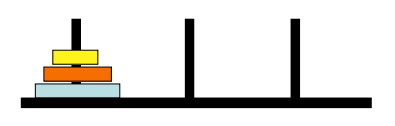
\includegraphics[scale = 0.3]{images/hanoi1}
    \caption{Towers of Hanoi with 3 disks}
  \label{fig1}
\end{figure}

\subsection{Questions}
\subsubsection*{1. Explain the method by which each of the two planners finds a solution}

\subsubsection*{2. Which planner was fastest?}
\subsubsection*{3. Explain why the winning planner might be more effective on this problem}

%-----------------------------------End of Problem 1 ---------------------------------------------%

\section{Project Part I: Sokoban PDDL}
%Assigned to Luis%
\begin{figure}[h!]
  \centering
    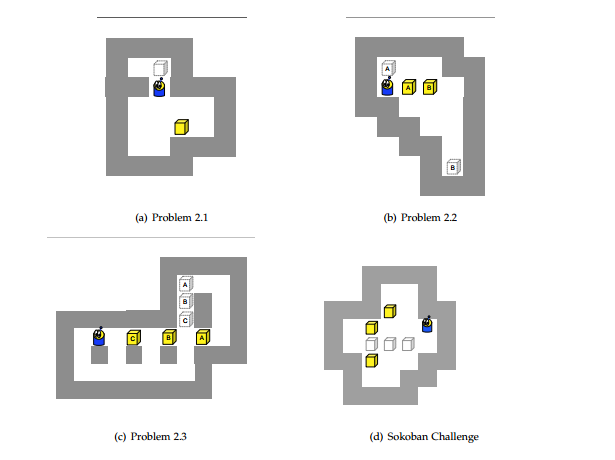
\includegraphics[scale = 0.3]{images/sokoban}
    \caption{Sokoban Problems}
  \label{fig2}
\end{figure}

\subsection{Questions}
\subsubsection*{1. Show successful plans from at least one planner on the three Sokoban problems in Figure \ref{fig2}
(1-3). The challenge problem is optional}
\subsubsection*{2. Compare the performance of two planners on this domain. Which one works better? Does this
make sense, why?}
\subsubsection*{3. Clearly PDDL was not intended for this sort of application. Discuss the challenges in expressing geometric constraints in semantic planning}
\subsubsection*{4. In many cases, geometric and dynamic planning are insufficient to describe a domain. Give
an example of a problem that is best suited for semantic (classical) planning. Explain why a
semantic representation would be desirable}

%------------------------------------End of Problem 2 -------------------------------------------------%

\section{Project Part II: Sokoban Planner}
%Assigned to James and Stango%
\subsection{Questions}
\subsubsection*{1. Give successful plans from your planner on the Sokoban problems in Figure \ref{fig2} and any others}
\subsubsection*{2. Compare the performance of your planner to the PDDL planners you used in the previous
problem. Which was faster? Why?}
\subsubsection*{3. Prove that your planner was complete. Your instructor has a math background: a proof ``is
a convincing argument.'' Make sure you address each aspect of completeness and why your
planner satisfies it. Pictures are always welcome.}
\subsubsection*{4. What methods did you use to speed up the planning? Give a short description of each method
and explain why it did or didn't help on each relevant problem}

%---------------------------------End of Problem 3 ----------------------------------------------------%

\section{Post-Project: Towers of Hanoi Revisited}
%Assigned to Arvind%
\subsection{Questions}
\subsubsection*{1. Give successful plans from at least one planner with 6 and 10 disks}
\subsubsection*{2. Do you notice anything about the structure of the plans? Can you use this to increase the
efficiency of planning for Towers of Hanoi? Explain}
\subsubsection*{In a paragraph or two, explain a general planning strategy that would take advantage of
problem structure. Make sure your strategy applies to problems other than Towers of Hanoi.
Would such a planner still be complete?}

%----------------------------------End of Problem 4 ----------------------------------------------------%

\bibliographystyle{unsrt}
\bibliography{myrefs}
\end{document}